% This must be in the first 5 lines to tell arXiv to use pdfLaTeX, which is strongly recommended.
\pdfoutput=1
% In particular, the hyperref package requires pdfLaTeX in order to break URLs across lines.

\documentclass[11pt]{article}

% Change "review" to "final" to generate the final (sometimes called camera-ready) version.
% Change to "preprint" to generate a non-anonymous version with page numbers.
% \usepackage[review]{acl}
\usepackage[final]{acl}

% Standard package includes
\usepackage{times}
\usepackage{latexsym}

% For proper rendering and hyphenation of words containing Latin characters (including in bib files)
\usepackage[T1]{fontenc}
% For Vietnamese characters
% \usepackage[T5]{fontenc}
% See https://www.latex-project.org/help/documentation/encguide.pdf for other character sets

% This assumes your files are encoded as UTF8
\usepackage[utf8]{inputenc}

% This is not strictly necessary, and may be commented out,
% but it will improve the layout of the manuscript,
% and will typically save some space.
\usepackage{microtype}
\usepackage{comment}
% This is also not strictly necessary, and may be commented out.
% However, it will improve the aesthetics of text in
% the typewriter font.
\usepackage{inconsolata}

%Including images in your LaTeX document requires adding
%additional package(s)
\usepackage{graphicx}
\usepackage{array}
\usepackage{multirow}
\usepackage{booktabs}
\usepackage{multirow}
\usepackage{graphicx}
\usepackage{subcaption}
\usepackage{amsmath}
\usepackage{booktabs}
\usepackage{listings}
\usepackage{xcolor}
\usepackage{tabularx}
\usepackage{booktabs}
\usepackage{colortbl}
\usepackage{soul}
\usepackage{pifont}


\newcommand{\todo}[1]{\textcolor{purple}{#1}}
\newcommand{\jjcomment}[1]{\textcolor{blue}{[~Jing: #1~]}}

% If the title and author information does not fit in the area allocated, uncomment the following
%
%\setlength\titlebox{<dim>}
%
% and set <dim> to something 5cm or larger.

\title{CAMI: A Counselor Agent Supporting Motivational Interviewing through State Inference and Topic Exploration}
% Aek's suggestions:
% Improving Motivational Interviewing Outcomes in LLM-Based Counselor Agents through State Estimation and Topic Exploration
% Improving LLM-Based Motivational Interviewing Agents Beyond Turn-Level Strategies with State Estimation and Topic Exploration
% An LLM-Based Motivational Interviewing Agent with Personalized State Estimation and Change Talk Exploration
% A Novel Framework for LLM-Based Motivational Interviewing Agents Using Topic Trees for Change Talk Exploration
% Enhancing Change Talk Exploration and Evocation in LLM-Based Counselor Agents with Topic Trees

% Author information can be set in various styles:
% For several authors from the same institution:
% \author{Author 1 \and ... \and Author n \\
%         Address line \\ ... \\ Address line}
% if the names do not fit well on one line use
%         Author 1 \\ {\bf Author 2} \\ ... \\ {\bf Author n} \\
% For authors from different institutions:
% \author{Author 1 \\ Address line \\  ... \\ Address line
%         \And  ... \And
%         Author n \\ Address line \\ ... \\ Address line}
% To start a separate ``row'' of authors use \AND, as in
% \author{Author 1 \\ Address line \\  ... \\ Address line
%         \AND
%         Author 2 \\ Address line \\ ... \\ Address line \And
%         Author 3 \\ Address line \\ ... \\ Address line}

% \author{First Author \\
%   Affiliation / Address line 1 \\
%   Affiliation / Address line 2 \\
%   Affiliation / Address line 3 \\
%   \texttt{email@domain} \\\And
%   Second Author \\
%   Affiliation / Address line 1 \\
%   Affiliation / Address line 2 \\
%   Affiliation / Address line 3 \\
%   \texttt{email@domain} \\}

\author{
 \textbf{Yizhe Yang\textsuperscript{1}~\thanks{Work was done during a visit at SMU.}},
 \textbf{Palakorn Achananuparp\textsuperscript{2}},
 \textbf{Heyan Huang\textsuperscript{1}~\thanks{Corresponding Author}},
 \textbf{Jing Jiang\textsuperscript{3}},
\\
 \textbf{Kit Phey Leng \textsuperscript{4}},
 \textbf{Nicholas Gabriel Lim \textsuperscript{5}},
 \textbf{Cameron Tan Shi Ern \textsuperscript{6}},
 \textbf{Ee-peng Lim\textsuperscript{2}}
\\
\\
 \textsuperscript{1}Beijing Institute of Technology,
 \textsuperscript{2}Singapore Management University,
 \textsuperscript{3}Australian National University, 
 \\
 \textsuperscript{4}National Institute of Education,
 \textsuperscript{5}Singapore University of Social Sciences,
 \textsuperscript{6}National University of Singapore
\\
 \small{
   % \textbf{Correspondence:} \href{mailto:email@domain}{email@domain}
   \{yizheyang,hhy63\}@bit.edu.cn, \{palakorna,eplim\}@smu.edu.sg, jing.jiang@anu.edu.au
 }
}

\begin{document}
\maketitle
\begin{abstract}
Conversational counselor agents have become essential tools for addressing the rising demand for scalable and accessible mental health support. This paper introduces 
CAMI, a novel automated counselor agent grounded in Motivational Interviewing (MI) -- a client-centered counseling approach designed to address ambivalence and facilitate behavior change.  
CAMI employs a novel STAR framework, consisting of client's state inference, motivation topic exploration, and response generation modules, leveraging large language models (LLMs). These components work together to evoke change talk, aligning with MI principles and improving counseling outcomes for clients from diverse backgrounds.
We evaluate CAMI’s performance through both automated and manual evaluations, utilizing simulated clients to assess MI skill competency, client's state inference accuracy, topic exploration proficiency, and overall counseling success. 
Results show that CAMI not only outperforms several state-of-the-art methods but also shows more realistic counselor-like behavior. Additionally, our ablation study underscores the critical roles of state inference and topic exploration in achieving this performance.

\end{abstract}

\section{Introduction}
\label{sec:introduction}
The business processes of organizations are experiencing ever-increasing complexity due to the large amount of data, high number of users, and high-tech devices involved \cite{martin2021pmopportunitieschallenges, beerepoot2023biggestbpmproblems}. This complexity may cause business processes to deviate from normal control flow due to unforeseen and disruptive anomalies \cite{adams2023proceddsriftdetection}. These control-flow anomalies manifest as unknown, skipped, and wrongly-ordered activities in the traces of event logs monitored from the execution of business processes \cite{ko2023adsystematicreview}. For the sake of clarity, let us consider an illustrative example of such anomalies. Figure \ref{FP_ANOMALIES} shows a so-called event log footprint, which captures the control flow relations of four activities of a hypothetical event log. In particular, this footprint captures the control-flow relations between activities \texttt{a}, \texttt{b}, \texttt{c} and \texttt{d}. These are the causal ($\rightarrow$) relation, concurrent ($\parallel$) relation, and other ($\#$) relations such as exclusivity or non-local dependency \cite{aalst2022pmhandbook}. In addition, on the right are six traces, of which five exhibit skipped, wrongly-ordered and unknown control-flow anomalies. For example, $\langle$\texttt{a b d}$\rangle$ has a skipped activity, which is \texttt{c}. Because of this skipped activity, the control-flow relation \texttt{b}$\,\#\,$\texttt{d} is violated, since \texttt{d} directly follows \texttt{b} in the anomalous trace.
\begin{figure}[!t]
\centering
\includegraphics[width=0.9\columnwidth]{images/FP_ANOMALIES.png}
\caption{An example event log footprint with six traces, of which five exhibit control-flow anomalies.}
\label{FP_ANOMALIES}
\end{figure}

\subsection{Control-flow anomaly detection}
Control-flow anomaly detection techniques aim to characterize the normal control flow from event logs and verify whether these deviations occur in new event logs \cite{ko2023adsystematicreview}. To develop control-flow anomaly detection techniques, \revision{process mining} has seen widespread adoption owing to process discovery and \revision{conformance checking}. On the one hand, process discovery is a set of algorithms that encode control-flow relations as a set of model elements and constraints according to a given modeling formalism \cite{aalst2022pmhandbook}; hereafter, we refer to the Petri net, a widespread modeling formalism. On the other hand, \revision{conformance checking} is an explainable set of algorithms that allows linking any deviations with the reference Petri net and providing the fitness measure, namely a measure of how much the Petri net fits the new event log \cite{aalst2022pmhandbook}. Many control-flow anomaly detection techniques based on \revision{conformance checking} (hereafter, \revision{conformance checking}-based techniques) use the fitness measure to determine whether an event log is anomalous \cite{bezerra2009pmad, bezerra2013adlogspais, myers2018icsadpm, pecchia2020applicationfailuresanalysispm}. 

The scientific literature also includes many \revision{conformance checking}-independent techniques for control-flow anomaly detection that combine specific types of trace encodings with machine/deep learning \cite{ko2023adsystematicreview, tavares2023pmtraceencoding}. Whereas these techniques are very effective, their explainability is challenging due to both the type of trace encoding employed and the machine/deep learning model used \cite{rawal2022trustworthyaiadvances,li2023explainablead}. Hence, in the following, we focus on the shortcomings of \revision{conformance checking}-based techniques to investigate whether it is possible to support the development of competitive control-flow anomaly detection techniques while maintaining the explainable nature of \revision{conformance checking}.
\begin{figure}[!t]
\centering
\includegraphics[width=\columnwidth]{images/HIGH_LEVEL_VIEW.png}
\caption{A high-level view of the proposed framework for combining \revision{process mining}-based feature extraction with dimensionality reduction for control-flow anomaly detection.}
\label{HIGH_LEVEL_VIEW}
\end{figure}

\subsection{Shortcomings of \revision{conformance checking}-based techniques}
Unfortunately, the detection effectiveness of \revision{conformance checking}-based techniques is affected by noisy data and low-quality Petri nets, which may be due to human errors in the modeling process or representational bias of process discovery algorithms \cite{bezerra2013adlogspais, pecchia2020applicationfailuresanalysispm, aalst2016pm}. Specifically, on the one hand, noisy data may introduce infrequent and deceptive control-flow relations that may result in inconsistent fitness measures, whereas, on the other hand, checking event logs against a low-quality Petri net could lead to an unreliable distribution of fitness measures. Nonetheless, such Petri nets can still be used as references to obtain insightful information for \revision{process mining}-based feature extraction, supporting the development of competitive and explainable \revision{conformance checking}-based techniques for control-flow anomaly detection despite the problems above. For example, a few works outline that token-based \revision{conformance checking} can be used for \revision{process mining}-based feature extraction to build tabular data and develop effective \revision{conformance checking}-based techniques for control-flow anomaly detection \cite{singh2022lapmsh, debenedictis2023dtadiiot}. However, to the best of our knowledge, the scientific literature lacks a structured proposal for \revision{process mining}-based feature extraction using the state-of-the-art \revision{conformance checking} variant, namely alignment-based \revision{conformance checking}.

\subsection{Contributions}
We propose a novel \revision{process mining}-based feature extraction approach with alignment-based \revision{conformance checking}. This variant aligns the deviating control flow with a reference Petri net; the resulting alignment can be inspected to extract additional statistics such as the number of times a given activity caused mismatches \cite{aalst2022pmhandbook}. We integrate this approach into a flexible and explainable framework for developing techniques for control-flow anomaly detection. The framework combines \revision{process mining}-based feature extraction and dimensionality reduction to handle high-dimensional feature sets, achieve detection effectiveness, and support explainability. Notably, in addition to our proposed \revision{process mining}-based feature extraction approach, the framework allows employing other approaches, enabling a fair comparison of multiple \revision{conformance checking}-based and \revision{conformance checking}-independent techniques for control-flow anomaly detection. Figure \ref{HIGH_LEVEL_VIEW} shows a high-level view of the framework. Business processes are monitored, and event logs obtained from the database of information systems. Subsequently, \revision{process mining}-based feature extraction is applied to these event logs and tabular data input to dimensionality reduction to identify control-flow anomalies. We apply several \revision{conformance checking}-based and \revision{conformance checking}-independent framework techniques to publicly available datasets, simulated data of a case study from railways, and real-world data of a case study from healthcare. We show that the framework techniques implementing our approach outperform the baseline \revision{conformance checking}-based techniques while maintaining the explainable nature of \revision{conformance checking}.

In summary, the contributions of this paper are as follows.
\begin{itemize}
    \item{
        A novel \revision{process mining}-based feature extraction approach to support the development of competitive and explainable \revision{conformance checking}-based techniques for control-flow anomaly detection.
    }
    \item{
        A flexible and explainable framework for developing techniques for control-flow anomaly detection using \revision{process mining}-based feature extraction and dimensionality reduction.
    }
    \item{
        Application to synthetic and real-world datasets of several \revision{conformance checking}-based and \revision{conformance checking}-independent framework techniques, evaluating their detection effectiveness and explainability.
    }
\end{itemize}

The rest of the paper is organized as follows.
\begin{itemize}
    \item Section \ref{sec:related_work} reviews the existing techniques for control-flow anomaly detection, categorizing them into \revision{conformance checking}-based and \revision{conformance checking}-independent techniques.
    \item Section \ref{sec:abccfe} provides the preliminaries of \revision{process mining} to establish the notation used throughout the paper, and delves into the details of the proposed \revision{process mining}-based feature extraction approach with alignment-based \revision{conformance checking}.
    \item Section \ref{sec:framework} describes the framework for developing \revision{conformance checking}-based and \revision{conformance checking}-independent techniques for control-flow anomaly detection that combine \revision{process mining}-based feature extraction and dimensionality reduction.
    \item Section \ref{sec:evaluation} presents the experiments conducted with multiple framework and baseline techniques using data from publicly available datasets and case studies.
    \item Section \ref{sec:conclusions} draws the conclusions and presents future work.
\end{itemize}

\section{RELATED WORK}
\label{sec:relatedwork}
In this section, we describe the previous works related to our proposal, which are divided into two parts. In Section~\ref{sec:relatedwork_exoplanet}, we present a review of approaches based on machine learning techniques for the detection of planetary transit signals. Section~\ref{sec:relatedwork_attention} provides an account of the approaches based on attention mechanisms applied in Astronomy.\par

\subsection{Exoplanet detection}
\label{sec:relatedwork_exoplanet}
Machine learning methods have achieved great performance for the automatic selection of exoplanet transit signals. One of the earliest applications of machine learning is a model named Autovetter \citep{MCcauliff}, which is a random forest (RF) model based on characteristics derived from Kepler pipeline statistics to classify exoplanet and false positive signals. Then, other studies emerged that also used supervised learning. \cite{mislis2016sidra} also used a RF, but unlike the work by \citet{MCcauliff}, they used simulated light curves and a box least square \citep[BLS;][]{kovacs2002box}-based periodogram to search for transiting exoplanets. \citet{thompson2015machine} proposed a k-nearest neighbors model for Kepler data to determine if a given signal has similarity to known transits. Unsupervised learning techniques were also applied, such as self-organizing maps (SOM), proposed \citet{armstrong2016transit}; which implements an architecture to segment similar light curves. In the same way, \citet{armstrong2018automatic} developed a combination of supervised and unsupervised learning, including RF and SOM models. In general, these approaches require a previous phase of feature engineering for each light curve. \par

%DL is a modern data-driven technology that automatically extracts characteristics, and that has been successful in classification problems from a variety of application domains. The architecture relies on several layers of NNs of simple interconnected units and uses layers to build increasingly complex and useful features by means of linear and non-linear transformation. This family of models is capable of generating increasingly high-level representations \citep{lecun2015deep}.

The application of DL for exoplanetary signal detection has evolved rapidly in recent years and has become very popular in planetary science.  \citet{pearson2018} and \citet{zucker2018shallow} developed CNN-based algorithms that learn from synthetic data to search for exoplanets. Perhaps one of the most successful applications of the DL models in transit detection was that of \citet{Shallue_2018}; who, in collaboration with Google, proposed a CNN named AstroNet that recognizes exoplanet signals in real data from Kepler. AstroNet uses the training set of labelled TCEs from the Autovetter planet candidate catalog of Q1–Q17 data release 24 (DR24) of the Kepler mission \citep{catanzarite2015autovetter}. AstroNet analyses the data in two views: a ``global view'', and ``local view'' \citep{Shallue_2018}. \par


% The global view shows the characteristics of the light curve over an orbital period, and a local view shows the moment at occurring the transit in detail

%different = space-based

Based on AstroNet, researchers have modified the original AstroNet model to rank candidates from different surveys, specifically for Kepler and TESS missions. \citet{ansdell2018scientific} developed a CNN trained on Kepler data, and included for the first time the information on the centroids, showing that the model improves performance considerably. Then, \citet{osborn2020rapid} and \citet{yu2019identifying} also included the centroids information, but in addition, \citet{osborn2020rapid} included information of the stellar and transit parameters. Finally, \citet{rao2021nigraha} proposed a pipeline that includes a new ``half-phase'' view of the transit signal. This half-phase view represents a transit view with a different time and phase. The purpose of this view is to recover any possible secondary eclipse (the object hiding behind the disk of the primary star).


%last pipeline applies a procedure after the prediction of the model to obtain new candidates, this process is carried out through a series of steps that include the evaluation with Discovery and Validation of Exoplanets (DAVE) \citet{kostov2019discovery} that was adapted for the TESS telescope.\par
%



\subsection{Attention mechanisms in astronomy}
\label{sec:relatedwork_attention}
Despite the remarkable success of attention mechanisms in sequential data, few papers have exploited their advantages in astronomy. In particular, there are no models based on attention mechanisms for detecting planets. Below we present a summary of the main applications of this modeling approach to astronomy, based on two points of view; performance and interpretability of the model.\par
%Attention mechanisms have not yet been explored in all sub-areas of astronomy. However, recent works show a successful application of the mechanism.
%performance

The application of attention mechanisms has shown improvements in the performance of some regression and classification tasks compared to previous approaches. One of the first implementations of the attention mechanism was to find gravitational lenses proposed by \citet{thuruthipilly2021finding}. They designed 21 self-attention-based encoder models, where each model was trained separately with 18,000 simulated images, demonstrating that the model based on the Transformer has a better performance and uses fewer trainable parameters compared to CNN. A novel application was proposed by \citet{lin2021galaxy} for the morphological classification of galaxies, who used an architecture derived from the Transformer, named Vision Transformer (VIT) \citep{dosovitskiy2020image}. \citet{lin2021galaxy} demonstrated competitive results compared to CNNs. Another application with successful results was proposed by \citet{zerveas2021transformer}; which first proposed a transformer-based framework for learning unsupervised representations of multivariate time series. Their methodology takes advantage of unlabeled data to train an encoder and extract dense vector representations of time series. Subsequently, they evaluate the model for regression and classification tasks, demonstrating better performance than other state-of-the-art supervised methods, even with data sets with limited samples.

%interpretation
Regarding the interpretability of the model, a recent contribution that analyses the attention maps was presented by \citet{bowles20212}, which explored the use of group-equivariant self-attention for radio astronomy classification. Compared to other approaches, this model analysed the attention maps of the predictions and showed that the mechanism extracts the brightest spots and jets of the radio source more clearly. This indicates that attention maps for prediction interpretation could help experts see patterns that the human eye often misses. \par

In the field of variable stars, \citet{allam2021paying} employed the mechanism for classifying multivariate time series in variable stars. And additionally, \citet{allam2021paying} showed that the activation weights are accommodated according to the variation in brightness of the star, achieving a more interpretable model. And finally, related to the TESS telescope, \citet{morvan2022don} proposed a model that removes the noise from the light curves through the distribution of attention weights. \citet{morvan2022don} showed that the use of the attention mechanism is excellent for removing noise and outliers in time series datasets compared with other approaches. In addition, the use of attention maps allowed them to show the representations learned from the model. \par

Recent attention mechanism approaches in astronomy demonstrate comparable results with earlier approaches, such as CNNs. At the same time, they offer interpretability of their results, which allows a post-prediction analysis. \par



\section{Temporal Representation Alignment}
\label{sec:approach}

When training a series of short-horizon goal-reaching and instruction-following tasks, our goal is to learn a representation space such that our policy can generalize to a new (long-horizon) task that can be viewed as a sequence of known subtasks.
We propose to structure this representation space by aligning the representations of states, goals, and language in a way that is more amenable to compositional generalization.

\paragraph{Notation.}
We take the setting of a goal- and language-conditioned MDP $\cM$ with state space $\cS$, continuous action space $\cA \subseteq (0,1)^{d_{\cA}}$, initial state distribution $p_0$, dynamics $\p(s'\mid s,a)$, discount factor $\gamma$, and language task distribution $p_{\ell}$.
A policy $\pi(a\mid s)$ maps states to a distribution over actions. We inductively define the $k$-step (action-conditioned) policy visitation distribution as:
\begin{align*}
    p^{\pi}_{1}(s_{1} \mid s_1, a_{1})
    &\triangleq p(s_1 \mid s_1, a_1),\\
    p^{\pi}_{k+1}(s_{k+1} \mid s_1, a_1)
    &\triangleq \nonumber\\*
      &\mspace{-120mu} \int_{\cA}\int_{\cS} p(s_{k+1} \mid s,a) \dd p^{\pi}_{k}(s \mid s_{1},a_1) \dd
        \pi(a \mid s)\\
    p^{\pi}_{k+t}(s_{k+t} \mid s_t,a_t)
    &\triangleq p^{\pi}(s_{k} \mid s_1, a_1) . \eqmark
        \label{eq:successor_distribution}
\end{align*}
Then, the discounted state visitation distribution can be defined as the distribution over $s^{+}$\llap, the state reached after $K\sim \operatorname{Geom}(1-\gamma)$ steps:
\begin{equation}
    p^{\pi}_{\gamma}(s^{+}  \mid  s,a) \triangleq \sum_{k=0}^{\infty} \gamma^{k} p^{\pi}_{k}(s^{+} \mid s,a).
    \label{eq:discounted_state_visitation}
\end{equation}

We assume access to a dataset of expert demonstrations $\cD = \{\tau_{i},\ell_i\}_{i=1}^{K}$, where each trajectory
\begin{equation}
    \tau_{i} = \{s_{t,i},a_{t,i}\}_{t=1}^{H} \in \cS \times \cA
    \label{eq:trajectory}
\end{equation}
is gathered by an expert policy $\expert$, and is then annotated with $p_{\ell}(\ell_{i} \mid s_{1,i}, s_{H,i})$.
Our aim is to learn a policy $\pi$ that can select actions conditioned on a new language instruction $\ell$.
As in prior work~\citep{walke2023bridgedata}, we handle the continuous action space by representing both our policy and the expert policy as an isotropic Gaussian with fixed variance; we will equivalently write $\pi(a\mid s, \varphi)$ or denote the mode as $\hat{a} = \pi(s,\varphi)$ for a task $\varphi$.

\begin{rebuttal}
    \subsection{Representations for Reaching Distant Goals}
    \label{sec:reaching_goals}

    We learn a goal-conditioned policy $\pi(a\mid s,g)$ that selects actions to reach a goal $g$ from expert demonstrations with behavioral cloning.
    Suppose we directly selected actions to imitate the expert on two trajectories in $\cD$:
    
    \begin{equation}
        \mspace{-100mu}\begin{tikzcd}[remember picture,sep=small]
            s_1 \rar & s_2 \rar  & \ldots \rar & s_{H} \rar & w      \quad \\
            w \rar   & s_1' \rar & \ldots \rar & s_{H}' \rar & g\quad
        \end{tikzcd}
        \begin{tikzpicture}[remember picture,overlay] \coordinate (a) at (\tikzcdmatrixname-1-5.north east);
            \coordinate (b) at (\tikzcdmatrixname-2-5.south east);
            \coordinate (c) at (a|-b);
            \draw[decorate,line width=1.5pt,decoration={brace,raise=3pt,amplitude=5pt}]
        (a) -- node[right=1.5em] {$\tau_{i}\in \cD$} (c); \end{tikzpicture}
        \label{eq:trajectory_diagram}
    \end{equation}
    When conditioned with the composed goal $g$, we would be unable to imitate effectively
        as the composed state-goal $(s,g)$ is jointly out of the training distribution.

    What \emph{would} work for reaching $g$ is to first condition the policy on the intermediate waypoint $w$, then upon reaching $w$, condition on the goal $g$, as the state-goal pairs $(s_{i},w)$, $(w,g)$, and $(s_{i}',g)$ are all in the training distribution.
    If we condition the policy on some intermediate waypoint distribution $p(w)$ (or sufficient statistics thereof) that captures all of these cases, we can stitch together the expert behaviors to reach the goal $g$.

    Our approach is to learn a representation space that captures this ability, so that a GCBC objective used in this space can effectively imitate the expert on the composed task.
     We begin with the goal-conditioned behavioral cloning~\citep{kaelbling1993learning}
        loss $\cL_{\textsc{bc}}^{\phi,\psi,\xi}$ conditioned with waypoints $w$.
    \begin{equation}
        \cL_{\textsc{bc}}\bigl(\{s_{i},a_{i},s_{i}^{+},g_{i}\}_{i=1}^{K}\bigr) = \sum_{{i=1}}^{K} \log \pi\bigl(a_{i} \mid s_{i},\psi(g_{i})\bigr).
        \label{eq:goal_conditioned_bc}
    \end{equation}
    Enforcing the invariance needed to stitch \cref{eq:trajectory_diagram} then reduces to aligning \mbox{$\psi(g) \leftrightarrow \psi(w).$}
    The temporal alignment objective $\phi(s)\leftrightarrow \phi(s^{+})$ accomplishes this indirectly by aligning both $\psi(w)$ and $\psi(g)$ to the shared waypoint representation $\phi(w)$:

    \csuse{color indices}
    \begin{align}
        &\cL_{\textsc{nce}}\bigl(\{s_{i},s_{i}^{+}\}_{i=1}^{K};\phi,\psi\bigr) =
        \log \biggl( {\frac{e^{\phi(s^+_{\i})^{T}\psi(s_{\i})}}{\sum_{{\j=1}}^{K}
                e^{\phi(s^+_{\i})^{T}\psi(s_{\j})}}} \biggr)  \nonumber\\*
                &\mspace{100mu} +
        \sum_{{\j=1}}^{K} \log \biggl( {\frac{e^{\phi(s^+_{\i})^{T}\psi(s_{\i})}}{\sum_{{\i=1}}^{K}
                e^{\phi(s^+_{\i})^{T}\psi(s_{\j})}}} \biggr)
        \label{eq:goal_alignment}
    \end{align}

        
\end{rebuttal}
\subsection{Interfacing with Language Instructions}
\label{sec:language_instructions}

To extend the representations from \cref{sec:reaching_goals} to compositional instruction following with language tasks, we need some way to ground language into the $\psi$ (future state)
representation space.
We use a similar approach to GRIF~\citep{myers2023goal}, which uses an additional CLIP-style \citep{radford2021learning} contrastive alignment loss with an additional pretrained language encoder $\xi$:
\csuse{no color indices}
\begin{align}
    &\cL_{\textsc{nce}}\bigl(\{g_{i},\ell_{i}\}_{i=1}^{K};\psi,\xi\bigr)
    = \sum_{{i=1}}^{K} \log \biggl( {\frac{e^{\psi(g_{\i})^{T}\xi(\ell_{\i})}}{\sum_{{\j=1}}^{K}
            e^{\psi(g_{\i})^{T}\xi(\ell_{\j})}}} \biggr)  \nonumber\\*
            &\mspace{100mu} +
    \sum_{{\j=1}}^{K} \log \biggl( {\frac{e^{\psi(g_{\i})^{T}\xi(\ell_{\i})}}{\sum_{{\i=1}}^{K}
            e^{\psi(g_{\i})^{T}\xi(\ell_{\j})}}} \biggr)
    \label{eq:task_alignment}
\end{align}

\subsection{Temporal Alignment}
\label{sec:temporal_alignment}

Putting together the objectives from \cref{sec:reaching_goals,sec:language_instructions} yields the Temporal Representation Alignment (\Method) approach.
\Method{} structures the representation space of goals and language instructions to better enable compositional generalization.
We learn encoders $\phi, \psi ,$ and $\xi$ to map states, goals, and language instructions to a shared representation space.

\csuse{color indices}
\begin{align}
    \cL_{\textsc{nce}} \label{eq:NCE}
    &(\{x_{i}, y_{i}\}_{i=1}^{K};f,h) =
        \sum_{{\i=1}}^{K} \log \biggl( {\frac{e^{f(y_{\i})^{T}h(x_{\i})}}{\sum_{{\j=1}}^{K}
        e^{f(y_{\i})^{T}h(x_{\j})}}} \biggr) \nonumber\\*
      &\mspace{100mu} +
        \sum_{{\j=1}}^{K} \log \biggl( {\frac{e^{f(y_{\i})^{T}h(x_{\i})}}{\sum_{{\i=1}}^{K}
        e^{f(y_{\i})^{T}h(x_{\j})}}} \biggr) \\
    \cL_{\textsc{bc}} \label{eq:BC}
    &\bigl(\{s_{i},a_{i},s^{+}_{i},\ell_{i}\}_{i=1}^{K};\pi,\psi,\xi\bigr) = \nonumber\\*
      &\mspace{-10mu} \sum_{{i=1}}^{K} \log
        \pi\bigl(a_{i} \mid s_{i},\xi(\ell_{i})\bigr) + \log \pi\bigl(a_{i} \mid
        s_{i},\psi(s^{+}_{i})\bigr) \\
    \cL_{\textsc{tra}}
    &\label{eq:TRA} \bigl( \{s_{i},a_{i},s_{i}^{+},g_{i},\ell_{i}\}_{i=1}^{K}; \pi,\phi,\psi,\xi\bigr)
        \\
    &= \underbrace{\cL_{\textsc{bc}}\bigl(\{s_{i},a_{i},s_{i}^{+},\ell_{i}\}_{i=1}^{K};\pi,\psi,\xi\bigr)}_{\text{behavioral
    cloning}} \nonumber\\*
    &+
        \underbrace{\cL_{\textsc{nce}}\bigl(\{s_{i},s_{i}^{+}\}_{i=1}^{K};\phi,\psi\bigr)}_{\text{temporal alignment}}
        + \underbrace{\cL_{\textsc{nce}}\bigl(\{g_{i},\ell_{i}\}_{i=1}^{K};\psi,\xi\bigr)}_{\text{task alignment}} \nonumber
\end{align}Note that the NCE alignment loss uses a CLIP-style symmetric contrastive objective~\citep{radford2021learning,eysenbach2024inference} \-- we highlight the indices in the NCE alignment loss~\eqref{eq:NCE} for clarity.

Our overall objective is to minimize \cref{eq:TRA} across states, actions, future states, goals, and language tasks within the training data:
\begin{align}
    &\min_{\pi,\phi,\psi,\xi} \mathbb{E}_{\substack{(s_{1,i},a_{1,i},\ldots,s_{H,i},a_{H,i},\ell) \sim \mathcal{D} \\
    i\sim\operatorname{Unif}(1\ldots H) \\
    k\sim\operatorname{Geom}(1-\gamma)}} \\*
    &\mspace{10mu}
    \Bigl[\cL_{\text{TRA}}\bigl(\{s_{t,i},a_{t,i},s_{\min(t+k,H),i},s_{H,i},\ell\}_{i=1}^{K};\pi,\phi,\psi,\xi\bigr)\Bigr].
    \label{eq:overall_objective}
\end{align}

\begin{algorithm}
    \caption{Temporal Representation Alignment}
    \label{alg:tra}
    \begin{algorithmic}[1]
        \State \textbf{input:} dataset $\mathcal{D} = (\{s_{t,i},a_{t,i}\}_{t=1}^{H},\ell_i)_{i=1}^N$
        \State initialize networks $\Theta \triangleq (\pi,\phi,\psi,\xi)$
        \While{training}
        \State sample batch $\bigl\{(s_{t,i},a_{t,i},s_{t+k,i},\ell_i)\bigr\}_{i=1}^K\sim\mathcal{D}$ \\
        \hspace*{2ex} for $k\sim\operatorname{Geom}(1-\gamma)$
        \State $\Theta \gets \Theta - \alpha \nabla_{\Theta} \cL_{\text{TRA}}\bigl(\{s_{t,i},a_{t,i},s_{t+k,i},\ell_i\}_{i=1}^K; \Theta\bigr)$
        \EndWhile
        \smallskip
        \State \textbf{output:} \parbox[t]{\linewidth}{language-conditioned policy $\pi(a_{t} | s_{t}, \xi(\ell))$ \\
            goal-conditioned policy $\pi(a_{t} | s_{t}, \psi(g))$
        }
    \end{algorithmic}
\end{algorithm}

\subsection{Implementation}
\label{sec:implementation}

A summary of our approach is shown in \cref{alg:tra}.
In essence, TRA learns three encoders: $\phi$, which encodes states, $\psi$ which encodes future goals, and $\xi$ which encodes language instructions.
Contrastive losses are used to align state representations $\phi(s_{t})$ with future goal representations $\psi(s_{t+k})$, which are in turn aligned with equivalent language task specifications $\xi(\ell)$ when available.
We then learn a behavior cloning policy $\pi$ that can be conditioned on either the goal or language instruction through the representation $\psi(g)$ or $\xi(\ell)$, respectively.

\begin{rebuttal}
    \subsection{Temporal Alignment and Compositionality}
    \label{sec:compositionality}

    We will formalize the intuition from \cref{sec:reaching_goals} that \Method{} enables compositional generalization by considering the error on a ``compositional'' version of $\cD,$ denoted $\cD^{*}$.
    Using the notation from \cref{eq:trajectory}, we can say $\cD$ is distributed according to:
    \begin{align}
        &\cD \triangleq \cD^{H} \sim \prod_{i=1}^{K} p_0(s_{1,i}) p_{\ell}(\ell_{i} \mid s_{1,i}, s_{H,i})
            \nonumber\\*
          &\mspace{60mu} \prod_{t=1}^{H} \expert(a_{t,i} \mid s_{t,i}) \p(s_{t+1,i} \mid s_{t,i}, a_{t,i}) ,
            \label{eq:dataset_distribution}
    \end{align}
    or equivalently
    \begin{align}
            &\cD^{H} \sim \prod_{i=1}^{K} p_0(s_{1,i}) p_{\ell}(\ell_{i} \mid s_{1,i}, s_{H,i}) \nonumber\\*
            &\mspace{60mu} \prod_{t=1}^{H}
            e^{\sigma^2\|\expert(s_{t,i}) - a_{t,i}\|^2}\p(s_{t+1,i} \mid s_{t,i}, a_{t,i}) ,
            \label{eq:dataset_distribution_2}
    \end{align}
    by the isotropic Gaussian assumption.
    We will define $\cD^{*} \triangleq \cD^{H'}$ to be a longer-horizon version of $\cD$ extending the behaviors gathered under $\expert$ across a horizon $\alpha H \ge H' \ge H$ that additionally satisfies a ``time-isotropy'' property: the marginal distribution of the states is uniform across the horizon, i.e., $p_0(s_{1,i}) = p_0(s_{t,i})$ for all $t \in \{1\ldots H'\}$.

    We will relate the in-distribution imitation error $\textsc{Err}(\bullet; \cD)$ to the compositional out-of-distribution imitation error $\textsc{Err}(\bullet;\cD^{*})$.
    We define
    \begin{align}
        \textsc{Err}(\hat{\pi}; \tilde{\cD})
        &= \E_{\tilde{\cD}}\Bigl[\frac{1}{H}\sum_{t=1}^{H} \mathbb{E}_{\hat{\pi}}\left[\|\tilde{a}_{t,i} -
        \hat{\pi}(\tilde{s}_{t,i}, \tilde{s}_{H, i})\|^{2}/d_{\cA}\right]\Bigr] \nonumber\\
        &\quad \text{for} \quad \{\tilde{s}_{t,i},\tilde{a}_{t,i},\tilde{\ell}_{i}\}_{t=1}^{H} \sim
            \tilde{\cD}.
            \label{eq:imitation_error}
    \end{align}
    On the training dataset this is equivalent to the expected behavioral cloning loss from \cref{eq:BC}.

                            
    \begin{assumption}
        \label{asm:policy_factorization}
        The policy factorizes through inferred waypoints as:
\begin{align}
    &\textrm{goals: }\pi(a \mid s, g)
        = \nonumber\\*
      &\mspace{50mu} \int \pi(a\mid s, w) \p(s_{t}=w \mid s_{t+k}=g) \dd{w}
        \label{eq:goal-conditioned} \\
    &\textrm{language: } \pi(a \mid s, \ell)
        = \int \pi(a\mid s, w) \nonumber\\*
      &\mspace{20mu} \p(s_{t}=w \mid s_{t+k}=g) \p(s_{t+k}=g \mid \ell) \dd{w} \dd{g} ,
        \label{eq:language-conditioned}
        \end{align}
        where denote by $\pi(s,g)$ the MLE estimate of the action $a$.

    \end{assumption}

    \makerestatable
    \begin{theorem}
        \label{thm:compositionality}
        Suppose $\cD$ is distributed according to \cref{eq:dataset_distribution} and $\cD^{*}$ is distributed according to \cref{eq:dataset_distribution}.
        When $\gamma > 1-1/H$ and $\alpha > 1$, for optimal features $\phi$ and $\psi$ under \cref{eq:overall_objective}, we have
        \begin{gather}
            \textsc{Err}(\pi; \cD^{*}) \le \textsc{Err}(\pi; \cD) +  \frac{\alpha -1}{2 \alpha }+\Bigl(\frac{ \alpha - 2 }{2\alpha}\Bigr) \1 \{\alpha >2\}  .
            \label{eq:compositionality}
        \end{gather}
    \end{theorem}

    We can also define a notion of the language-conditioned compositional generalization error:
    \begin{equation*}
        \errl(\pi; \cD^{*}) \triangleq \E_{\cD^{*}}\Bigl[\frac{1}{H}\sum_{t=1}^{H}
            \mathbb{E}_{\pi}\bigl[\|\tilde{a}_{t,i} - \pi(\tilde{s}_{t,i}, \tilde{\ell}_{i})\|^{2}\bigr]\Bigr].
            \label{eq:language_error}
    \end{equation*}

    \makerestatable
    \begin{corollary}
        \label{thm:language}
        Under the same conditions as \cref{thm:compositionality},
        \begin{equation*}
            \errl(\pi; \cD^{*}) \le \errl(\pi; \cD) +  \frac{\alpha -1}{2 \alpha }+\Bigl(\frac{ \alpha - 2 }{2\alpha}\Bigr) \1 \{\alpha >2\}  .
            \label{eq:compositionality_language}
        \end{equation*}

    \end{corollary}

    The proofs as well as a visualization of the bound are in \cref{app:compositionality}. Policy implementation details can be found in \cref{app:tra_impl}

    
                
        
    \end{rebuttal}


\section{Experiments}
\label{sec:exp}
Following the settings in Section \ref{sec:existing}, we evaluate \textit{NovelSum}'s correlation with the fine-tuned model performance across 53 IT datasets and compare it with previous diversity metrics. Additionally, we conduct a correlation analysis using Qwen-2.5-7B \cite{yang2024qwen2} as the backbone model, alongside previous LLaMA-3-8B experiments, to further demonstrate the metric's effectiveness across different scenarios. Qwen is used for both instruction tuning and deriving semantic embeddings. Due to resource constraints, we run each strategy on Qwen for two rounds, resulting in 25 datasets. 

\subsection{Main Results}

\begin{table*}[!t]
    \centering
    \resizebox{\linewidth}{!}{
    \begin{tabular}{lcccccccccc}
    \toprule
    \multirow{3}*{\textbf{Diversity Metrics}} & \multicolumn{10}{c}{\textbf{Data Selection Strategies}} \\
    \cmidrule(lr){2-11}
    & \multirow{2}*{\textbf{K-means}} & \multirow{2}*{\vtop{\hbox{\textbf{K-Center}}\vspace{1mm}\hbox{\textbf{-Greedy}}}}  & \multirow{2}*{\textbf{QDIT}} & \multirow{2}*{\vtop{\hbox{\textbf{Repr}}\vspace{1mm}\hbox{\textbf{Filter}}}} & \multicolumn{5}{c}{\textbf{Random}} & \multirow{2}{*}{\textbf{Duplicate}} \\ 
    \cmidrule(lr){6-10}
    & & & & & \textbf{$\mathcal{X}^{all}$} & ShareGPT & WizardLM & Alpaca & Dolly &  \\
    \midrule
    \rowcolor{gray!15} \multicolumn{11}{c}{\textit{LLaMA-3-8B}} \\
    Facility Loc. $_{\times10^5}$ & \cellcolor{BLUE!40} 2.99 & \cellcolor{ORANGE!10} 2.73 & \cellcolor{BLUE!40} 2.99 & \cellcolor{BLUE!20} 2.86 & \cellcolor{BLUE!40} 2.99 & \cellcolor{BLUE!0} 2.83 & \cellcolor{BLUE!30} 2.88 & \cellcolor{BLUE!0} 2.83 & \cellcolor{ORANGE!20} 2.59 & \cellcolor{ORANGE!30} 2.52 \\    
    DistSum$_{cosine}$  & \cellcolor{BLUE!30} 0.648 & \cellcolor{BLUE!60} 0.746 & \cellcolor{BLUE!0} 0.629 & \cellcolor{BLUE!50} 0.703 & \cellcolor{BLUE!10} 0.634 & \cellcolor{BLUE!40} 0.656 & \cellcolor{ORANGE!30} 0.578 & \cellcolor{ORANGE!10} 0.605 & \cellcolor{ORANGE!20} 0.603 & \cellcolor{BLUE!10} 0.634 \\
    Vendi Score $_{\times10^7}$ & \cellcolor{BLUE!30} 1.70 & \cellcolor{BLUE!60} 2.53 & \cellcolor{BLUE!10} 1.59 & \cellcolor{BLUE!50} 2.23 & \cellcolor{BLUE!20} 1.61 & \cellcolor{BLUE!30} 1.70 & \cellcolor{ORANGE!10} 1.44 & \cellcolor{ORANGE!20} 1.32 & \cellcolor{ORANGE!10} 1.44 & \cellcolor{ORANGE!30} 0.05 \\
    \textbf{NovelSum (Ours)} & \cellcolor{BLUE!60} 0.693 & \cellcolor{BLUE!50} 0.687 & \cellcolor{BLUE!30} 0.673 & \cellcolor{BLUE!20} 0.671 & \cellcolor{BLUE!40} 0.675 & \cellcolor{BLUE!10} 0.628 & \cellcolor{BLUE!0} 0.591 & \cellcolor{ORANGE!10} 0.572 & \cellcolor{ORANGE!20} 0.50 & \cellcolor{ORANGE!30} 0.461 \\
    \midrule    
    \textbf{Model Performance} & \cellcolor{BLUE!60}1.32 & \cellcolor{BLUE!50}1.31 & \cellcolor{BLUE!40}1.25 & \cellcolor{BLUE!30}1.05 & \cellcolor{BLUE!20}1.20 & \cellcolor{BLUE!10}0.83 & \cellcolor{BLUE!0}0.72 & \cellcolor{ORANGE!10}0.07 & \cellcolor{ORANGE!20}-0.14 & \cellcolor{ORANGE!30}-1.35 \\
    \midrule
    \midrule
    \rowcolor{gray!15} \multicolumn{11}{c}{\textit{Qwen-2.5-7B}} \\
    Facility Loc. $_{\times10^5}$ & \cellcolor{BLUE!40} 3.54 & \cellcolor{ORANGE!30} 3.42 & \cellcolor{BLUE!40} 3.54 & \cellcolor{ORANGE!20} 3.46 & \cellcolor{BLUE!40} 3.54 & \cellcolor{BLUE!30} 3.51 & \cellcolor{BLUE!10} 3.50 & \cellcolor{BLUE!10} 3.50 & \cellcolor{ORANGE!20} 3.46 & \cellcolor{BLUE!0} 3.48 \\ 
    DistSum$_{cosine}$ & \cellcolor{BLUE!30} 0.260 & \cellcolor{BLUE!60} 0.440 & \cellcolor{BLUE!0} 0.223 & \cellcolor{BLUE!50} 0.421 & \cellcolor{BLUE!10} 0.230 & \cellcolor{BLUE!40} 0.285 & \cellcolor{ORANGE!20} 0.211 & \cellcolor{ORANGE!30} 0.189 & \cellcolor{ORANGE!10} 0.221 & \cellcolor{BLUE!20} 0.243 \\
    Vendi Score $_{\times10^6}$ & \cellcolor{ORANGE!10} 1.60 & \cellcolor{BLUE!40} 3.09 & \cellcolor{BLUE!10} 2.60 & \cellcolor{BLUE!60} 7.15 & \cellcolor{ORANGE!20} 1.41 & \cellcolor{BLUE!50} 3.36 & \cellcolor{BLUE!20} 2.65 & \cellcolor{BLUE!0} 1.89 & \cellcolor{BLUE!30} 3.04 & \cellcolor{ORANGE!30} 0.20 \\
    \textbf{NovelSum (Ours)}  & \cellcolor{BLUE!40} 0.440 & \cellcolor{BLUE!60} 0.505 & \cellcolor{BLUE!20} 0.403 & \cellcolor{BLUE!50} 0.495 & \cellcolor{BLUE!30} 0.408 & \cellcolor{BLUE!10} 0.392 & \cellcolor{BLUE!0} 0.349 & \cellcolor{ORANGE!10} 0.336 & \cellcolor{ORANGE!20} 0.320 & \cellcolor{ORANGE!30} 0.309 \\
    \midrule
    \textbf{Model Performance} & \cellcolor{BLUE!30} 1.06 & \cellcolor{BLUE!60} 1.45 & \cellcolor{BLUE!40} 1.23 & \cellcolor{BLUE!50} 1.35 & \cellcolor{BLUE!20} 0.87 & \cellcolor{BLUE!10} 0.07 & \cellcolor{BLUE!0} -0.08 & \cellcolor{ORANGE!10} -0.38 & \cellcolor{ORANGE!30} -0.49 & \cellcolor{ORANGE!20} -0.43 \\
    \bottomrule
    \end{tabular}
    }
    \caption{Measuring the diversity of datasets selected by different strategies using \textit{NovelSum} and baseline metrics. Fine-tuned model performances (Eq. \ref{eq:perf}), based on MT-bench and AlpacaEval, are also included for cross reference. Darker \colorbox{BLUE!60}{blue} shades indicate higher values for each metric, while darker \colorbox{ORANGE!30}{orange} shades indicate lower values. While data selection strategies vary in performance on LLaMA-3-8B and Qwen-2.5-7B, \textit{NovelSum} consistently shows a stronger correlation with model performance than other metrics. More results are provided in Appendix \ref{app:results}.}
    \label{tbl:main}
    \vspace{-4mm}
\end{table*}


\begin{table}[t!]
\centering
\resizebox{\linewidth}{!}{
\begin{tabular}{lcccc}
\toprule
\multirow{2}*{\textbf{Diversity Metrics}} & \multicolumn{3}{c}{\textbf{LLaMA}} & \textbf{Qwen}\\
\cmidrule(lr){2-4} \cmidrule(lr){5-5} 
& \textbf{Pearson} & \textbf{Spearman} & \textbf{Avg.} & \textbf{Avg.} \\
\midrule
TTR & -0.38 & -0.16 & -0.27 & -0.30 \\
vocd-D & -0.43 & -0.17 & -0.30 & -0.31 \\
\midrule
Facility Loc. & 0.86 & 0.69 & 0.77 & 0.08 \\
Entropy & 0.93 & 0.80 & 0.86 & 0.63 \\
\midrule
LDD & 0.61 & 0.75 & 0.68 & 0.60 \\
KNN Distance & 0.59 & 0.80 & 0.70 & 0.67 \\
DistSum$_{cosine}$ & 0.85 & 0.67 & 0.76 & 0.51 \\
Vendi Score & 0.70 & 0.85 & 0.78 & 0.60 \\
DistSum$_{L2}$ & 0.86 & 0.76 & 0.81 & 0.51 \\
Cluster Inertia & 0.81 & 0.85 & 0.83 & 0.76 \\
Radius & 0.87 & 0.81 & 0.84 & 0.48 \\
\midrule
NovelSum & \textbf{0.98} & \textbf{0.95} & \textbf{0.97} & \textbf{0.90} \\
\bottomrule
\end{tabular}
}
\caption{Correlations between different metrics and model performance on LLaMA-3-8B and Qwen-2.5-7B.  “Avg.” denotes the average correlation (Eq. \ref{eq:cor}).}
\label{tbl:correlations}
\vspace{-2mm}
\end{table}

\paragraph{\textit{NovelSum} consistently achieves state-of-the-art correlation with model performance across various data selection strategies, backbone LLMs, and correlation measures.}
Table \ref{tbl:main} presents diversity measurement results on datasets constructed by mainstream data selection methods (based on $\mathcal{X}^{all}$), random selection from various sources, and duplicated samples (with only $m=100$ unique samples). 
Results from multiple runs are averaged for each strategy.
Although these strategies yield varying performance rankings across base models, \textit{NovelSum} consistently tracks changes in IT performance by accurately measuring dataset diversity. For instance, K-means achieves the best performance on LLaMA with the highest NovelSum score, while K-Center-Greedy excels on Qwen, also correlating with the highest NovelSum. Table \ref{tbl:correlations} shows the correlation coefficients between various metrics and model performance for both LLaMA and Qwen experiments, where \textit{NovelSum} achieves state-of-the-art correlation across different models and measures.

\paragraph{\textit{NovelSum} can provide valuable guidance for data engineering practices.}
As a reliable indicator of data diversity, \textit{NovelSum} can assess diversity at both the dataset and sample levels, directly guiding data selection and construction decisions. For example, Table \ref{tbl:main} shows that the combined data source $\mathcal{X}^{all}$ is a better choice for sampling diverse IT data than other sources. Moreover, \textit{NovelSum} can offer insights through comparative analyses, such as: (1) ShareGPT, which collects data from real internet users, exhibits greater diversity than Dolly, which relies on company employees, suggesting that IT samples from diverse sources enhance dataset diversity \cite{wang2024diversity-logD}; (2) In LLaMA experiments, random selection can outperform some mainstream strategies, aligning with prior work \cite{xia2024rethinking,diddee2024chasing}, highlighting gaps in current data selection methods for optimizing diversity.



\subsection{Ablation Study}


\textit{NovelSum} involves several flexible hyperparameters and variations. In our main experiments, \textit{NovelSum} uses cosine distance to compute $d(x_i, x_j)$ in Eq. \ref{eq:dad}. We set $\alpha = 1$, $\beta = 0.5$, and $K = 10$ nearest neighbors in Eq. \ref{eq:pws} and \ref{eq:dad}. Here, we conduct an ablation study to investigate the impact of these settings based on LLaMA-3-8B.

\begin{table}[ht!]
\centering
\resizebox{\linewidth}{!}{
\begin{tabular}{lccc}
\toprule
\textbf{Variants} & \textbf{Pearson} & \textbf{Spearman} & \textbf{Avg.} \\
\midrule
NovelSum & 0.98 & 0.96 & 0.97 \\
\midrule
\hspace{0.10cm} - Use $L2$ distance & 0.97 & 0.83 & 0.90\textsubscript{↓ 0.08} \\
\hspace{0.10cm} - $K=20$ & 0.98 & 0.96 & 0.97\textsubscript{↓ 0.00} \\
\hspace{0.10cm} - $\alpha=0$ (w/o proximity) & 0.79 & 0.31 & 0.55\textsubscript{↓ 0.42} \\
\hspace{0.10cm} - $\alpha=2$ & 0.73 & 0.88 & 0.81\textsubscript{↓ 0.16} \\
\hspace{0.10cm} - $\beta=0$ (w/o density) & 0.92 & 0.89 & 0.91\textsubscript{↓ 0.07} \\
\hspace{0.10cm} - $\beta=1$ & 0.90 & 0.62 & 0.76\textsubscript{↓ 0.21} \\
\bottomrule
\end{tabular}
}
\caption{Ablation Study for \textit{NovelSum}.}
\label{tbl:ablation}
\vspace{-2mm}
\end{table}

In Table \ref{tbl:ablation}, $\alpha=0$ removes the proximity weights, and $\beta=0$ eliminates the density multiplier. We observe that both $\alpha=0$ and $\beta=0$ significantly weaken the correlation, validating the benefits of the proximity-weighted sum and density-aware distance. Additionally, improper values for $\alpha$ and $\beta$ greatly reduce the metric's reliability, highlighting that \textit{NovelSum} strikes a delicate balance between distances and distribution. Replacing cosine distance with Euclidean distance and using more neighbors for density approximation have minimal impact, particularly on Pearson's correlation, demonstrating \textit{NovelSum}'s robustness to different distance measures.







\section{Conclusion}
In this paper, we address the challenges of using LLMs to create counselor agents that practice motivational interviewing style counseling using our proposed STAR framework.  This framework includes client's state inference, topic exploration for change talk, and MI-adherent strategy selection.  Based on the framework, we develop CAMI a counselor agent that engages clients in change talks making positive changes to their behaviors. By extracting motivation topics and their superclass relationships from AnnoMI dataset and Wikipedia knowledge base, we construct a novel topic tree covering hierarchical motivation topics that can be navigated by CAMI as it explores the topics of change talk for clients having diverse profiles. Furthermore, CAMI selects strategies from MI skills to generate strategy-aligned responses. Extensive experiments and analyses, including automated and expert user evaluations, show that the STAR framework underlying CAMI effectively guides LLMs to adhere to MI techniques. CAMI also outperforms state-of-the-art counseling agents in our comprehensive evaluation, reducing the gap between human and AI-based counseling. 

\section*{Limitations}
Although CAMI shows promising results in MI-based counseling, we could identify three main limitations which can be addressed in the future work.

Firstly, our work has not studied how sensitive is CAMI to the multiple steps of prompting due to the accumulation of generation errors. Even though some aspects of the performance, such as topic exploration, are not optimal, we believe that other methods could be implemented to improve module performance while maintaining the novelty and effectiveness of the overall framework. Designing effective prompts and evaluating their performance are therefore important areas for further research. 

Secondly, our framework currently relies on LLM prompting to perform state inference, topic exploration and strategy selection. Our human experts have raised concerns about issues related to strategy use, such as counselor responses being too lengthy and using too many questions. In our future work, we would therefore plan to enhance the strategy selection module further such as incorporating the idea of action rules introduced in DIIR. 

Finally, our study focuses on MI-based counseling and the AnnoMI dataset.  However, the proposed STAR framework can be adapted to other counseling techniques, such as Cognitive Behavioral Therapy (CBT), and relevant counseling datasets.  Future research could explore the integration of MI and CBT techniques within a single counselor agent, potentially enhancing the counseling effectiveness. 

\section*{Ethical Considerations}
This work does not advocate for the direct use of LLMs in therapy. Although our proposed CAMI system outperforms previous methods and demonstrates proficiency in MI techniques, it still falls short of the expertise provided by high-quality human counselors. Therefore, we do not suggest that LLMs should replace the role of human counselors. While the outputs of LLMs are certainly not as specialized or accurate as those of professionals, they can serve as supplementary tools to support and inspire human-led exploration. Our goal is to provide an alternative approach for applying LLMs in psychological support, offering ideas that may spark further discussions and development in the field of NLP and psychology. We believe this can help advance future research in AI applications for psychology and sociology. Moreover, while MI techniques aim to facilitate positive change, system deployers should carefully assess the topics covered to mitigate potential risks. Additionally, users interacting with systems incorporating MI abilities should be informed of the system's identity, ensuring they are aware of the nature of their interaction and can make an informed choice.


% Bibliography entries for the entire Anthology, followed by custom entries
%\bibliography{anthology,custom}
% Custom bibliography entries only
\bibliography{custom}

\appendix

\section{Detailed Implementation}
\label{app:implement}

In this section, we provide the detailed implementation of our method and experiment evaluation, which includes the prompts and instructions for human evaluation. We set the top-p and temperature parameters to 0.7 and 0.8 respectively for ChatGPT to generate more diverse responses, while setting the top-p and temperature parameters to 0.2 and 0.3 respectively for GPT-4 to achieve more precise predictions.

\subsection{States, Actions \& Receptivity}

Table~\ref{tab:state desciption}, Table~\ref{tab:action description} and Table~\ref{tab:receptivity description} cover the descriptions of states, actions and different levels of receptivity respectively. %{\color{orange} These descriptions will be used in the following prompts.}{\color{red} (What?)}. 


\begin{table*}[tb]
\centering
\begin{tabularx}{\textwidth}{lXp{4cm}}
\toprule
State            & Description                                                                                                                                  & Relevant Actions                                    \\ \midrule
Precontemplation & The client is unaware of or underestimates the need for change.           & Inform, Engage, Deny, \newline Blame, Downplay     \\ \hline
Contemplation    & The client acknowledges the need for change but remains ambivalent.     & Inform, Engage, Hesitate, \newline  Doubt, Acknowledge    \\ \hline
Preparation      & The client is ready to act, planning specific steps toward change.                                        & Inform, Engage, Reject, \newline Accept, Plan\\ \hline
Termination      & In the final stage of counseling, the client gradually ends the conversation.                                                     & Terminate     \\ \bottomrule
\end{tabularx}
\caption{The states of change and corresponding actions used in our simulation framework.}
\label{tab:state desciption}
\end{table*}


\begin{table*}[tb]
\centering
\begin{tabularx}{\textwidth}{lX}
\toprule
Action      & Description                                                                                                                                      \\ \midrule
Deny        & The client directly refuses to admit their behavior is problematic or needs change.                                                              \\ \hline
Downplay    & The client downplays the importance or impact of their behavior or situation.                                                                    \\ \hline
Blame       & The client attributes their issues to external factors, such as stressful life or other people.                                                  \\ \hline
Hesitate    & The client shows uncertainty, indicating ambivalence about change.                                                                               \\ \hline
Doubt       & The client expresses skepticism about the practicality or success of proposed changes.                                                           \\ \hline
Engage      & The client interacts politely with the counselor, such as greeting, thanking or ask questions.                                                   \\ \hline
Inform      & The client shares details about their background, experiences, or emotions.                                                                      \\ \hline
Acknowledge & The client highlight the importance, benefit or confidence to change.                                                                            \\ \hline
Accept      & The client agrees to adopt the suggested action plan.                                                                                            \\ \hline
Reject      & The client declines the proposed plan, deeming it unsuitable.                                                                                    \\  \hline
Plan        & The client proposes or details steps for a change plan.                                                                                          \\ \hline
Terminate   & The client highlights current state, expresses a desire to end the current session, and suggests further discussion be deferred to a later time. \\ \bottomrule
\end{tabularx}
\caption{Actions Used in Our Framework.}
\label{tab:action description}
\end{table*}

\begin{table*}[tb]
\centering
\begin{tabularx}{\textwidth}{lX}
\toprule
Receptivity                     & Description                                                                                                                                                                                                                                                                                                      \\ \midrule
High receptivity (5)            & A client with high receptivity consistently demonstrates behaviors such as frequently and openly sharing personal thoughts and feelings, actively engaging in discussions about change, quickly and positively responding to suggestions, and displaying strong self-belief in their ability to make changes. \\ \hline
Moderately High receptivity (4) & Clients with moderately high receptivity are generally open and forthcoming, mostly receptive to change discussions, respond well to suggestions with occasional need for reinforcement, and demonstrate good self-belief with some need for reassurance.                                                     \\ \hline
Moderate receptivity (3)        & Clients with moderate receptivity show a balance between sharing and withholding information, exhibit mixed interest in change discussions, respond to suggestions neutrally, and display a balanced view of their ability to change.                                                                         \\ \hline
Moderately Low receptivity (2)  & Clients with moderately low receptivity are characterized by reluctance to share personal information, limited interest in change discussions, resistance to suggestions, and low self-belief with frequent expression of doubts.                                                                             \\ \hline
Low receptivity (1)             & Clients with low receptivity consistently withhold information, avoid discussions about change, strongly resist suggestions, and show very low self-belief, often highlighting reasons why change is not possible.                                                                                            \\ \bottomrule
\end{tabularx}
\caption{Receptivity at Different Levels in Our Framework.}
\label{tab:receptivity description}
\end{table*}


\subsection{Simulated Counselor and Moderator}

To realize our proposed framework, we evaluate client simulation methods in a set of synthetically generated counseling sessions involving both a simulated counselor and a simulated moderator. The latter manages the conversation between the client and counselor agents so as to determine when to end the counseling session. Since this work focuses on client simulation, we adopt prompting-based implementations for both the counselor and moderator agents, as shown in Table~\ref{tab:couneslor prompt} and Table~\ref{tab:moderator prompt} respectively. Unlike that for counselor simulation, the prompt for moderator simulation adopts a few-shot approach to perform in-context learning so as to answer the question of whether to conclude the session.  Five positive examples and five negative examples were included in the few-shot demonstration. To ensure a fair evaluation of different simulated clients, we employed the same counselor agent and moderator agent for all generated sessions. 

%Previous studies, such as \citep{yosef2024assessing,wang2024towards}, have demonstrated the effectiveness of LLM-based counselor agents in MI counseling. Therefore, we utilized a counselor agent built upon state-of-the-art research to evaluate clients. {\color{orange}To design the moderator demonstration, we initially conducted a preliminary experiment involving both an LLM and a human acting as the moderator. During generation, the generation process concluded based on the judgment of the LLM moderator in a zero-shot manner. Subsequently, we collected 50 generated session snippets and annotated whether the session was concluded correctly or not manually. Of these, 37 were concluded correctly, which we labeled as positive examples, while the remaining 13 were incorrectly concluded by the LLM moderator, which we labeled as negative examples. Upon manual inspection, the majority of failures were attributed to the counselor misjudging the client’s state or the client expressing negative impacts rather than motivation. We selected five positive examples and five negative examples as the few-shot demonstration for the final moderator. Subsequently, the accuracy of the LLM moderator reaches 88\% in the second round experiment, which is satisfactory. }{\color{red} (One session generated by both LLM and human moderators? How are the positive/negative examples determined?)} 
% {\color{red} (EP: I thought we want mention that using the same simulated counselor and moderator agents in the generated conversations with different clients simulated by different methods is a reasonably fair evaluation approach.  I wonder how we extract the examples for the moderator prompt. They should not be full conversations.)}


\begin{table*}[tb]
\centering
\begin{tabularx}{\textwidth}{lX}
\toprule
Prompt Type     & Prompt \\ \midrule
System Prompt & Motivational interviewing (MI) is a client-centered counseling approach designed to facilitate behavioral change by resolving ambivalence and enhancing motivation. As a counselor, you should guide the conversation through the following stages:\newline 1. Engage: Begin by exploring the client’s background and emotional state with open-ended questions. This builds rapport and helps understand their perspective without immediately focusing on change.\newline 2. Identify Behavioral Issues: Transition to identifying behaviors the client might consider changing. Employ reflective listening to grasp their concerns and aspirations fully.\newline 3. Motivate Change: Guide the conversation towards reasons for altering problematic behaviors. Utilize affirmations, summaries, and reflections to bolster their motivation, avoiding any forceful imposition of your viewpoints. Never directly ask about the motivation.\newline 4. Address Concerns: After motivating the client, they may still express concerns and hesitations. Engage with these apprehensions, seeking to address them constructively.\newline 5. Action Plan: Once the client is ready, collaborate to formulate a detailed action plan. This should include achievable steps that reinforce their commitment and support their choices, enhancing their sense of ownership over the change process.\newline \newline In the following conversation, you will play as a Counselor in a counselling conversation with Client. Reply with only utterance of Counselor and Keep utterances natural and succinct, mimicking a real conversation. Start your utterances with 'Counselor:'. \\ \hline
Assistant     & Counselor: Hello. How are you?                                                                                                           \\ \hline
User          & Client: I am good. What about you?                                                                          \\ \hline
...           & ...                                                                                                      \\ \bottomrule
\end{tabularx}
\caption{Prompt for Counselor Simulation: The prompt ends with starting off the session with predefined first utterances of the simulated counselor and client agents.}
\label{tab:couneslor prompt}
\end{table*}

\begin{table*}[tb]
\begin{tabularx}{\textwidth}{X}
\toprule
Your task is to assess the current state of the conversation (the most recent utterances) and determine whether the conversation has concluded.\newline The conversation is considered to have concluded if any of the following conditions are met:\newline - The Client and Counselor work out an actionable plan together.\newline - The Counselor decides not to pursue any changes in the Client's behavior and communicates readiness to provide support in the future.\newline \newline Here are some examples to help you understand the task better:\newline [examples]\newline \newline \newline Here is a new Conversation Snippet:\newline [context]\newline \newline Question: Should the conversation be concluded?  \\ \bottomrule
\end{tabularx}
\caption{Prompt for Moderator Simulation in the Few-Shot Format. The [examples] section is to be replaced by real examples annotated by human and the [context] section is to be replaced by the conversation so far.}
\label{tab:moderator prompt}
\end{table*}

\subsection{Baseline Methods}
\label{app:baselines}

Tables~\ref{tab:baseclient prompt}, ~\ref{tab:example based prompt}, ~\ref{tab:profile based prompt} and ~\ref{tab:action based prompt} show the prompts for the baseline methods, i.e., Base method, Example-based method, Profile-based method and Pro+Act-based method respectively.

\begin{table*}[tb]
\begin{tabularx}{\textwidth}{lX}
\toprule
Prompt Type     & Prompt \\ \midrule
System Prompt & In this role-play scenario, you will be assuming the role of a Client engaged in a conversation with a Counselor. The Counselor's objective is to guide and potentially persuade you about your [behavioral problem]. The essence of this exercise is to simulate a realistic and dynamic interaction. Keep utterance natural and succinct, mimicking a real conversation and start your utterance with 'Client'. \\ \hline
User         & Counselor: Hello. How are you?                                                                                                           \\ \hline
Assistant          & Client: I am good. What about you?                                                                          \\ \hline
...           & ...                 \\ \bottomrule
\end{tabularx}
\caption{Prompt for the Base Client in a chatting format. The [behavioral problem] section is to be replaced by the behavioral problem description in the client profile.}
\label{tab:baseclient prompt}
\end{table*}

\begin{table*}[tb]
\begin{tabularx}{\textwidth}{lX}
\toprule
Prompt Type     & Prompt \\ \midrule
System Prompt &  You will be provided with a conversation between a client and a counselor. Your task is to simulate the same client talking to a different therapist in a parallel universe. You can ignore that the previous chat ever happened. While the context of the previous conversation should not influence this session, it should guide you on how the client communicates, including their tone of speech, sentence structure, and the manner in which they address particular topics or concerns. Essentially, you're creating a new conversation but with the client's life situation and their response pattern maintained. Only generate the client utterances started by "Client: ". Here is the provided conversation: \newline [conversation]  \\ \hline
User         & Counselor: Hello. How are you?                                                                                                           \\ \hline
Assistant    & Client: I am good. What about you?                                                                          \\ \hline
...           & ...             \\ \bottomrule
\end{tabularx}
\caption{Prompt for the Example-based Client in a chatting format. The [conversation] section is to be replaced by the real conversation.}
\label{tab:example based prompt}
\end{table*}


\begin{table*}[tb]
\begin{tabularx}{\textwidth}{lX}
\toprule
Prompt Type     & Prompt \\ \midrule
System Prompt & You are speaking with a motivational interviewing counselor therapist, and you are the client in this conversation with the following personal information: \newline [profile] \newline \newline You should follow the previous information to act as a client in the conversation. Your responses should be coherent and avoid repeating previous utterances. In your response, please avoid repeating expressions of gratitude or similar sentiments multiple times if you’ve already expressed them during the conversation. Your response should start with "Client: " and only include part of what the Client should say!  \\ \hline
User         & Counselor: Hello. How are you?                                                                                                           \\ \hline
Assistant    & Client: I am good. What about you?                                                                          \\ \hline
...           & ...                     \\ \bottomrule
\end{tabularx}
\caption{Prompt for the Profile-based Client in a chatting format. The [profile] section is to be replaced by the profile of client.}
\label{tab:profile based prompt}
\end{table*}


\begin{table*}[tb]
\begin{tabularx}{\textwidth}{lX}
\toprule
Prompt Type     & Prompt \\ \midrule
System Prompt & You are speaking with a motivational interviewing counselor, and you are the client in this conversation with the following personal information: \newline [profile] \newline \#\# Instruction \newline You must follow the instructions below during chat.  \newline 1. Your utterances and behavior need to strictly follow your persona. Varying your wording and avoid repeating yourself verbatim!  \newline 2. You can decide to change your state and attitude flexibly based on your persona and the conversation. \newline 3. Only reply with one utterance of the simulated client. DO NOT generate the whole conversation. \newline \newline  \newline \#\# Your Response Actions  \newline 1. "Deny": Directly refuse to admit their behavior is problematic or needs change without additional reasons. \newline 2. "Downplay": Downplay the importance or impact of their behavior or situation. \newline 3. "Blame": Blame external factors or others to justify their behavior. \newline 4. "Inform": Share details about their background, experiences, or emotions. \newline 5. "Engage": Interacts politely with the counselor, such as greeting or thanking. \newline 6. "Hesitate": Show uncertainty, indicating ambivalence about change. \newline 7. "Doubt": Express skepticism about the practicality or success of proposed changes. \newline 8. "Acknowledge": Acknowledge the need for change. \newline 9. "Accept": Agree to adopt the suggested action plan. \newline 10. "Reject": Decline the proposed plan, deeming it unsuitable. \newline 11. "Plan": Propose or detail steps for a change plan. \newline  \newline You should follow the previous information to act as a client in the conversation. Your responses should be coherent and avoid repeating previous utterances. In your response, please avoid repeating expressions of gratitude or similar sentiments multiple times if you’ve already expressed them during the conversation. Your response should start with "Client: " and only include part of what the Client should say!  \\ \hline
User         & Counselor: Hello. How are you?                                                                                                           \\ \hline
Assistant    & Client: I am good. What about you?                                                                          \\ \hline
...           & ...             \\ \bottomrule
\end{tabularx}

\caption{Prompt for the Action-based Client in a chatting format. The [profile] section is to be replaced by the profile of client.}
\label{tab:action based prompt}
\end{table*}


\subsection{Methods for the Components of Our Framework}
\label{app:our frame implement}

Tables~\ref{tab:state transition prompt1}, \ref{tab:state transition prompt2}, \ref{tab:action selection prompt}, \ref{tab:information slection prompt}, and \ref{tab:generation prompt} provide prompts for implementing the state transition, context-aware action distribution, information selection and utterance generation methods in our proposed framework respectively.

\begin{table*}[tb]
\begin{tabularx}{\textwidth}{X}
\toprule
You task is to assess the alignment of the Counselor's utterances to the Client's motivation regarding a specific topic to determine whether the Counselor has mention the Client's motivation. \newline  Analysis Steps: \newline 1. Interpretation of the Counselor's Statement Briefly: Examine the Counselor's statement thoroughly to understand its content and focus, particularly regarding what reasons or aspects the Counselor proposed to explore in the Client's motivation. \newline 2. Clarification of the Client's Motivation: Elaborate on the Client’s specific motivation for the topic, such as body health, family relationships, etc. \newline 3. Assessment of Alignment: Determine to what extent the Counselor's statement **directly** mentioned the Client's motivation. Focus on alignment with specific motivations (such as health) rather than the generalized topic (such as reducing alcohol consumption). \newline 4. Justification of Assessment: Provide a comprehensive justification for your assessment. Analyze the connections between the Counselor’s statement and the Client's motivation, and conclude with a percentage score that indicates to what extent the Client's motivations are mentioned (e.g., 80\%). If the Counselor hasn't explicitly mentioned any specific reasons, the score should be 0\%. \newline Ensure that your analysis is logical, thorough, and well-supported, with clear justifications for each assessment step. \newline Here are some examples to help you understand the task better: \newline[examples] \newline Now, Here is the conversation snippet toward [topic]: \newline [context] \newline  The Motivation of Client is as follows: \newline [motivation] \newline Question: To what extent the Counselor's statement mention the Client's motivation?\\ \bottomrule
\end{tabularx}
\caption{Prompt for the state transition from Precontemplation to Contemplation in our framework. The [examples] will be replaced by some human annotated examples while [topic], [motivation], and [context] sections are to be replaced by the corresponding information.}
\label{tab:state transition prompt1}
\end{table*}

\begin{table*}[tb]
\begin{tabularx}{\textwidth}{X}
\toprule
Your task is to evaluate the alignment of the counselor's response to the client's concerns to determine whether the Counselor has resolved the Client's concern. \newline Analysis Steps: \newline 1. Clarification of the Client’s Hesitation: Elaborate on the client’s specific concerns as expressed in their hesitation regarding the topic. \newline 2. Interpretation of the Counselor's Statement: Examine the counselor’s statement thoroughly to discern its content and focus, particularly in relation to addressing the client’s concerns. \newline 3. Assessment of Alignment: Determine the extent to which the counselor’s statement addresses the client’s hesitations. Evaluate the directness and relevance of the response to the stated concerns. \newline 4. Justification of Assessment: Provide a detailed justification for your assessment of alignment. This should include an analysis of the connections (or lack thereof) between the counselor’s statement and the client’s reasons for hesitation. Conclude with a percentage score indicating the degree to which the client’s concerns are addressed (e.g., 80\%). \newline Ensure that your analysis is comprehensive and logically structured, offering clear and well-supported justifications for each assessment step. \newline Here are some examples to help you understand the task better: \newline [examples] \newline Now, Here is the conversation snippet toward [topic]:\newline[context] \newline The Client's concern is: [beliefs]\newline Question: To what extent the Counselor's statement relieve the Client's concern? \\ \bottomrule
\end{tabularx}
\caption{Prompt for the state transition from Contemplation to Preparation in our framework. The [examples] section is to be replaced by some human annotated examples while the [topic], [context] and [beliefs] sections are to be replaced by the corresponding information.}
\label{tab:state transition prompt2}
\end{table*}

\begin{table*}[tb]
\begin{tabularx}{\textwidth}{X}
\toprule
Assume you are a Client involved in a counseling conversation. The current conversation is provided below: \newline [context] \newline \newline  Based on the context, allocate probabilities to each of the following dialogue actions to maintain coherence: \newline [optional actions] \newline  Provide your response in JSON format, ensuring that the sum of all probabilities equals 100. 
\\ \bottomrule
\end{tabularx}
\caption{Prompt for the context-aware action distribution in our framework. The [context] section is to be replaced by the previous context while the [optional actions] section is to be replaced by actions set corresponding to the current state.}
\label{tab:action selection prompt}
\end{table*}

\begin{table*}[tb]
\begin{tabularx}{\textwidth}{X}
\toprule
Assume you are a Client engaged in a counseling conversation with a Counselor. You now in [station]. Your task is to choose the most appropriate persona/belief/plan. \newline Context of the Conversation: \newline [context] \newline  The Client's Personas/Beliefs/Plans: \newline [profile] \newline Action:  [action] \newline Based on the context and action, select the most appropriate persona/belief/plan (only one). Restate this reason using the original text.
\\ \bottomrule
\end{tabularx}
\caption{Prompt for the information selection in our framework. The [state], [context], and [action] sections are to be replaced by the current state, previous context and selected action, respectively. The [profile] section is to  be replaced by corresponding items in the client profile.}
\label{tab:information slection prompt}
\end{table*}

\begin{table*}[tb]
\begin{tabularx}{\textwidth}{lX}
\toprule
Prompt Type     & Prompt \\ \midrule
System Prompt & In this role-play, you'll assume the role of a Client discussing [topic]. Your responses should adhere to the following guidelines: \newline  - Begin each response with 'Client: '. \newline - Follow the predetermined actions enclosed in square brackets precisely. \newline - Ensure your response are coherent and avoid repeating previous utterances. \newline - Be natural and concise, but don't be overly polite. \newline Here is the overall profile given to you \newline [profile]  \\ \hline
User         & Counselor: Hello. How are you? {\color{blue} [State: The client is unaware of or underestimates the need for change., Action: The client interacts politely with the counselor, such as greeting, thanking or ask questions.]}                                                                                           \\ \hline
Assistant    & Client: I am good. What about you?                                                                          \\ \hline
...           & ...             \\ \bottomrule
\end{tabularx}

\caption{Prompt for the utterance generation of our framework in a chatting format. The [topic], and [profile] sections are to be replaced by the topic of counseling and profile of client. The text in {\color{blue} blue} is the format of instruction.}
\label{tab:generation prompt}
\end{table*}


\begin{table*}[!t]
    \small
    \centering
    \caption{Human evaluation results on  \textit{Long-MT-Bench+} using MPNet-based retrieval model. The response generation model is \texttt{GPT-3.5-Turbo}. 
    }
    \label{tab: human_evaluation}
    \resizebox{1\columnwidth}{!}{
    \begin{tabular}{l|cccccc}
    \toprule
    
    \textbf{Methods} & \textbf{Coherence} & \textbf{Consistency} & \textbf{Memorability} & \textbf{Engagingness} & \textbf{Humanness} & \textbf{Average} \\ 
    \midrule
    Full-History & 1.55 & 1.11 & 0.43 & 0.33 & 1.85 & 1.05 \\
    Sentence-Level & 1.89 & 1.20 & 1.06 & 0.78 & 2.00 & 1.39 \\
    Session-Level & 1.75 & 1.25 & 0.98 & 0.80 & 1.92 & 1.34 \\
    \midrule
    ConditionMem & 1.58 & 1.08 & 0.57 & 0.49 & 1.77 & 1.10 \\
    MemoChat & 2.05 & 1.25 & 1.12 & 0.86 & \textbf{2.10} & 1.48 \\
    COMEDY & \textbf{2.20} & 1.28 & 1.20 & 0.90 & 1.97 & 1.51 \\
    \midrule
    \sysname\ (Ours) & 2.13 & \textbf{1.34} & \textbf{1.28} & \textbf{0.94} & 2.06 & 1.55 \\

    \bottomrule
    \end{tabular}
    }
\end{table*}

% !TEX root = main.tex

\begin{figure}[t]
\vspace{-1.5cm}
\begin{minipage}{0.34\textwidth}
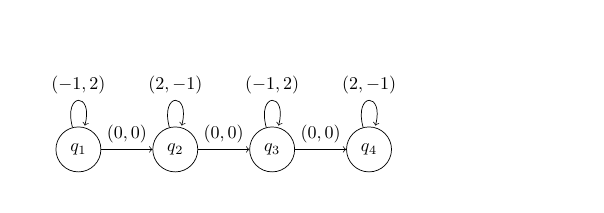
\begin{tikzpicture}[scale=0.25]
\usetikzlibrary{automata, positioning}
\scalebox{0.65}{
\node[state] (q1) {$q_1$};
\node[state, right=of q1] (q2) {$q_2$};
\node[state, right=of q2] (q3) {$q_3$};
\node[state, right=of q3] (q4) {$q_4$};

\path[->] (q1) edge [loop above] node[above] {$(-1,2)$} (q1) edge node[above] {$(0,0)$} (q2); 
\path[->] (q2) edge [loop above] node[above] {$(2,-1)$} (q2) edge node[above] {$(0,0)$} (q3);
\path[->] (q3) edge [loop above] node[above] {$(-1,2)$} (q3) edge node[above] {$(0,0)$} (q4);
\path[->] (q4) edge [loop above] node[above] {$(2,-1)$} (q4);
}
\end{tikzpicture}
\end{minipage}
\begin{minipage}{0.32\textwidth}
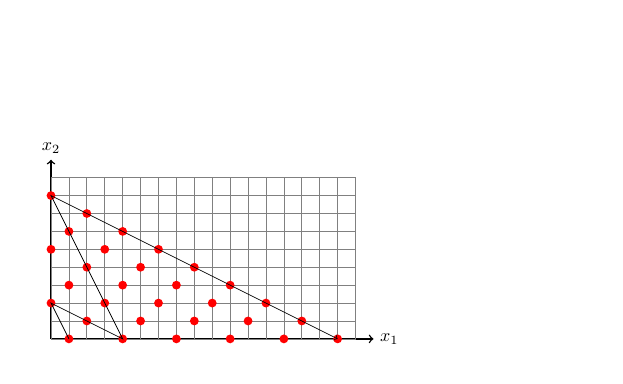
\begin{tikzpicture}[scale=0.35]
\scalebox{0.65}{
\draw[->, thick] (0, 0) -- (18, 0) node[right] {$x_1$};
\draw[->, thick] (0, 0) -- (0, 10) node[above] {$x_2$};

\draw[step=1, gray, thin] (0, 0) grid (17, 9);

\foreach \x in {1,4,7,10,13,16} \fill[red] (\x,0) circle (7pt);
\foreach \x in {2,5,8,11,14} \fill[red] (\x,1) circle (7pt);
\foreach \x in {0,3,6,9,12} \fill[red] (\x,2) circle (7pt);
\foreach \x in {1,4,7,10} \fill[red] (\x,3) circle (7pt);
\foreach \x in {2,5,8} \fill[red] (\x,4) circle (7pt);
\foreach \x in {0,3,6} \fill[red] (\x,5) circle (7pt);
\foreach \x in {1,4} \fill[red] (\x,6) circle (7pt);
\foreach \x in {2} \fill[red] (\x,7) circle (7pt);
\foreach \x in {0} \fill[red] (\x,8) circle (7pt);

\draw[->] (1,0) -- (0,2) -- (2,1) -- (4,0) -- (3,2) -- (2,4) -- (1,6) -- (0,8) -- (2,7) -- (4,6) -- (6,5) -- (8,4) -- (10,3) -- (12,2) -- (14,1) -- (16,0);
}
\end{tikzpicture}
\end{minipage}
\begin{minipage}{0.32\textwidth}
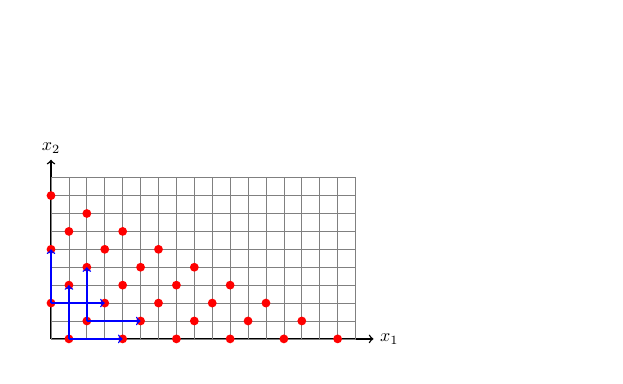
\begin{tikzpicture}[scale=0.35]
\scalebox{0.65}{
\draw[->, thick] (0, 0) -- (18, 0) node[right] {$x_1$};
\draw[->, thick] (0, 0) -- (0, 10) node[above] {$x_2$};

\draw[step=1, gray, thin] (0, 0) grid (17, 9);

\foreach \x in {1,4,7,10,13,16} \fill[red] (\x,0) circle (7pt);
\foreach \x in {2,5,8,11,14} \fill[red] (\x,1) circle (7pt);
\foreach \x in {0,3,6,9,12} \fill[red] (\x,2) circle (7pt);
\foreach \x in {1,4,7,10} \fill[red] (\x,3) circle (7pt);
\foreach \x in {2,5,8} \fill[red] (\x,4) circle (7pt);
\foreach \x in {0,3,6} \fill[red] (\x,5) circle (7pt);
\foreach \x in {1,4} \fill[red] (\x,6) circle (7pt);
\foreach \x in {2} \fill[red] (\x,7) circle (7pt);
\foreach \x in {0} \fill[red] (\x,8) circle (7pt);

\draw[->,blue,thick] (1,0) -- (4,0);
\draw[->,blue,thick] (1,0) -- (1,3);

\draw[->,blue,thick] (2,1) -- (5,1);
\draw[->,blue,thick] (2,1) -- (2,4);

\draw[->,blue,thick] (0,2) -- (3,2);
\draw[->,blue,thick] (0,2) -- (0,5);
}
\end{tikzpicture}
\end{minipage}
\caption{Left: 4-component \dvass $V_2$. 
Middle: the set $\reach_{q_4}(V_2, q_1(1,0))$ and a path $q_1(1,0) \tran q_4(16,0)$.
Right: bases 
%$A = \{(1,0),(2,1),(0,2)\}$ 
and periods 
%$P = \{(0,3),(3,0)\}$
 of an over-approximating semi-linear set $A+P^*$.}
\label{fig:zigzag}
\end{figure}

\begin{example}
For $k\geq 1$, let $V_k$ be a $(2k)$-component \dvass, where each component has just one state $q_i$
and one transition:
$(q_i, (-1,2), q_i)$ for odd $i$, and $(q_i, (2,-1), q_i)$ for even $i$.
Bridge transitions are $(q_i, (0,0), q_{i+1})$.
Figure~\ref{fig:zigzag} shows $V_2$ (left) and 
a path in $V_2$ from $s = q_1(1,0)$ to $t = q_4(16,0)$ together with 
the reachability set $\reach_{q_4}(V_2, s)$ (middle).
In general,
\begin{align} \label{eq:reachk}
X_k := \reach_{q_{2k}}(V_k, s) \ = \ \set{(x_1,x_2) \mid x_1+2x_2 \leq 4^k, \  x_1+2x_2 \equiv 1 \!\! \mod 3}.
\end{align}
Even if the size of the reachability set is 
exponential in $k$, for small $(x_1, x_2)$ it is periodic and the periods are small.
The set $X_k$ can be over-approximated by $A + P^*$ for $A = \set{(1,0),(2,1),(0,2)}$ and $P = \set{(0,3),(3,0)}$
(shown on the right of Figure~\ref{fig:zigzag}), namely for every $k\geq 1$ and $B\in\N$,
the set $X_k$ is \kanapka {$8$} {$B$}. 
For illustration, consider $Y := X_k \cap ((1,0) + P^*)$.
If $(1,0) + P^{\leq B} \subseteq X_k$ then $Y$ is a $B$-approximation
of $(1,0) + P^*$ with $\norm((1,0)), \norm(P) \leq 3 \leq 8$. 
Otherwise, there is some $(v_1, v_2) \in \big((1,0) + P^{\leq B}\big)\setminus X_k$, and
then $B$ is larger than $4^k$:
\[
%8B \geq 2(1 + 3B) \geq 2(v_1 + v_2) \geq v_1 + 2 v_2 > 
4^k < v_1 + 2 v_2 \leq 2(v_1 + v_2) \leq 2(1+3B) \leq 8B.
\]
Therefore by \eqref{eq:reachk}, each $(x_1,x_2) \in Y$ satisfies 
$\norm(x_1,x_2) = x_1 + x_2 \leq x_1 + 2x_2 \leq 4^k < 8B$, and thus
$Y$, seen as a union of singletons, is a union of 
linear sets with norm of base bounded by $8B$ and empty set of periods. 
In both cases, 
$Y$ is \kanapka {$8$} {$B$}. 
%The same intuition stays behind polynomial approximability of \dvass stated in Lemma~\ref{lem:2vass-sandwich}.
\end{example}

\end{document}
